\chapter{Background and Terminology}
\label{chp:background}

This chapter details event sourcing and related terminology. We provide an 
overview on benefits and constraints of event-sourced systems and examine 
in which cases event sourcing can be applied beneficially as a style of 
architecture. 
Furthermore, we describe Command Query Responsibility Segregation (CQRS), 
a complementary architectural style for event-sourced systems, and illustrate 
which benefits can be gained from applying it.

\begin{figure}[t]
	\centering
	\begin{subfigure}[t!]{0.29\textwidth}
        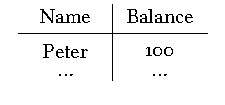
\includegraphics[width=\textwidth]
		{../illustrations/table.pdf}
	\caption{
		Active Record Example
	}
	\label{fig:table}
	\end{subfigure}
	%\quad
	\begin{subfigure}[t!]{0.67\textwidth}
	       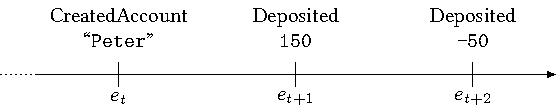
\includegraphics[width=\textwidth]
			{../illustrations/account-stream.pdf}
		\caption{
			Event Sourcing Example
		}
		\label{fig:log}
	\end{subfigure}
	\caption{Two different ways of storing the same current state.}
\end{figure}

\section{Active Record}
Many software systems require some kind of data management. A common approach
is to retain the current state of an application within some kind of data 
storage (e.g. a database) and return it on request. \emph{Active Record} is a 
software pattern which refers to the interaction with this current state (i.e. 
the active record) by applying create, read, update, or delete operations
(CRUD) on objects in a relational database (Figure \ref{fig:table}) 
\cite{Fowler2002}. 
In this approach, only the current state of an object is maintained and 
manipulated; previous values are overwritten and everything not saved is 
lost. This approach fits well for many applications but has shortcomings 
in terms of traceability and support for operations on the history.

\section{Event Sourcing}
\label{sec:es}
Most literature on event sourcing can be found online in blog posts, 
presentations, and software documentation. Academic literature on the 
topic is scarce.
This section provides an overview on how event sourcing is defined in
different resources and establishes the vocabulary used throughout this 
thesis.

\subsection{Different Definitions}
There is no standardized vocabulary on the topic, the terminology and 
definitions vary depending on the author. 

\paragraph{Martin Fowler}{
The term event sourcing was first established in a blog post by Martin 
Fowler \cite{Fowler2005} in 2005. 
He describes events as a series of changes in the state of an application. 
This series of events captures everything required to rebuild the current 
state. He views events as immutable and the event log as an append-only 
store. Events are never deleted, the only mean to revoke an event is a 
retroactive event~\cite{Fowler2005_2}. 
Once appended to the event log, this retroactive event acts as an inverse
event to a prior event and revokes its effects. 
%
Fowler does not distinguish clearly between events and the commands 
(i.e. actions) which triggered them.
This is an issue which is addressed in various works \cite{Chassaing2013, Reitzammer2013}.
}

\paragraph{Greg Young}{
Greg Young is another renowned author in the event sourcing domain. 
He describes event sourcing as ``storing [the] current state as a series of 
events and rebuilding state within the system by replaying that series of 
events'' \cite{Young2010}.
In his view, the event log possesses an append-only behavior as well: 
``[events] have already happened and cannot be undone'' \cite{Young2013}.
What Fowler calls retroactive events, Young describes as reversal
transactions \cite[p.31]{Young2013}.
}

\paragraph{Udi Dahan}{
Udi Dahan is a further author of a number of relevant blog posts and articles 
concerning event-sourced systems. To him, event sourcing refers to ``the state 
of the domain model being persisted as a stream of events rather than as a 
single snapshot [\dots]'' \cite{Betts2013}.
}

\paragraph{Martin Krasser}{
The articles and presentations by Martin Krasser concerning the persistence 
module in the Akka toolkit provide another view on event sourcing 
\mbox{\cite{Krasser2013, Krasser2015}.}
In this context, actors in a distributed system communicate via messages, 
which trigger state changes. Event sourcing is used as the mean to persist 
changes to the state of an actor.
State changes are ``appended as immutable facts to a journal'' \cite{Krasser2013}. 
A motivation for using it is that this approach ``allows for very high 
transaction rates and efficient replication''.
Recovering the state of an actor (e.g. after a restart or crash) is done by 
reapplying (i.e. replaying) the persisted events.
}


\ \\
The common ground of all these definitions is to publish every change to the 
state of an object (or system, or application) as an immutable event to an 
append-only event log. 
This results in a series of events, which when replayed always leads to the 
exact same state of the object (Figure \ref{fig:log}). Individual definitions 
vary or make no statement in terms of the editing semantics of the event log, 
the granularity of events, and the motivation for using it.

Where traditional architectures retain and maintain only the current state
of an object, event sourcing maintains all state-altering operations. Where 
CRUD offers four operations to apply modifications, event-sourced systems 
are restrained to only one operation: append-only.

\subsection{Benefits of Event Sourcing}
\label{sec:es-cs-benefits} 
An often found recommendation in literature is to apply event sourcing only in 
a clearly delimited part of a system and not force its usage upon a context 
where it does not appear beneficial \cite{Betts2013}.
A commonality often found in event-sourced systems, is that they possess a 
complex business logic. This is opposed to e.g. an application that provides 
``just'' an editing frontend to a relational database. We now briefly describe 
some of the benefits which an event-sourced architecture can provide.

\paragraph{Audit Log}{
In regulated areas (e.g. the financial industry), government regulations in 
many countries require companies to maintain records on the operation of a 
system. For example, the governmental regulations in the United States require 
brokers to keep their records in a non-rewriteable, non-erasable format \cite{sec17a}.
Event sourcing, with its append-only event log and immutable event characteristic, 
fits this requirement very well. Technologies such as write-once-read-many (WORM) 
data storages can be used complementarily with event sourcing.
If a WORM storage is used, the device prevents alterations of data in the hardware 
and allows only the appending of new data. 
}

\paragraph{Debugging}{
The captured events can be used to gain further insights into how the system 
reached its current states and which events were responsible for it. This is 
a strength in terms of traceability and debugging capabilities, since it makes 
it easier e.g. to retrace where a bug originated in a system.
}

\paragraph{Scalability}{
The append-only nature of an event log is thought to be beneficial for scalable 
architectures.
%
In such architectures it is common to have multiple replicated instances of the
same data model. These replications need to be kept in synchronization, in order 
to provide a consistent view on the data.
In event-sourced systems, the appending of events is the only mean to synchronize 
the replicated instances.
Due to fewer necessary locks, an append-only architecture with immutable events 
is thought to scale easier for reads than e.g. an architecture with a need for 
model synchronization via updates \cite[p.14-15]{Anderson2010}\cite{esdocs}.
}

\paragraph{Informative Value}{
Another motivation for applying event sourcing can be the informative value
(also sometimes referred to as ``business value''\footnote[1]{\href{http://docs.geteventstore.com/introduction/event-sourcing-basics/\#business-value-of-the-event-log}{http://docs.geteventstore.com/introduction/event-sourcing-basics/\#business-value-of-the-event-log}
}) of retrospectively examining the event log. All past states of a system 
can be reconstructed or queried. 
This can provide great value to systems, especially when the analysis of 
interaction with the system (e.g. customer behavior) is important. In such 
systems it is usually unknown what analysis one will execute in the future.
An example to illustrate this is an online shop where a shop administrator 
wants to list all products which have at some point been removed from a 
shopping cart. In event-sourced architectures, the state of the shopping 
cart at each past point can be queried.
}

\ \\
There are a number of documents describing how event sourcing has been applied 
in real-world systems. To highlight two information-rich documentations:
The financial trading platform LMAX utilizes event sourcing \cite{Fowler2011}
and a documentation published by the Microsoft Windows Azure team describes several 
case studies \cite{Betts2013}.
Furthermore, event-sourced frameworks like Akka\footnote[2]{\href{http://akka.io/}{http://akka.io/}}, 
Event Store\footnote[3]{\href{https://geteventstore.com/}{https://geteventstore.com/}}, or the Eventuate\footnote[4]{\href{https://rbmhtechnology.github.io/eventuate/}{https://rbmhtechnology.github.io/eventuate/}} 
toolkit by the Red Bull Media House provide the foundation for a number of 
real-world systems. 
 
\subsection{Thesis Terminology}
\label{sec:thesis-vocabulary}
Now that various authors' understanding of event sourcing has been described,
we establish the terminology used throughout this thesis. Since authors in the 
field use varying terminology, our terminology may differ from the individual 
authors' understanding.

\paragraph{Event}{
An event is a change to the state of an application. Each event is appended to 
the event log. It is important to note that the state change has already 
occurred to the entity. 
To reflect this, we name events as verbs in the past tense (e.g. \evt{ProductCreated}).
The granularity of events is defined through the context in which event sourcing 
is applied.
%
Events can be replayed in order to rebuild the state of a system up to a 
certain point. Except for the first event, each event builds upon the previous 
event. A replay process always needs to start from the beginning, though 
snapshots may be used as substitutions. 
}

\paragraph{Snapshot}
Snapshots are an established mean to optimize the process of restoring state. 
They represent the state of the system at a certain point in the event log 
and can be used instead of replaying the events prior to the snapshot.

\paragraph{Event Log}{
The event log provides the stream of all events which belong to an application.
An exchangeable term for the event log is the \emph{event stream}.
Figure \ref{fig:projections} depicts an excerpt of a hypothetical event log.

\begin{figure}[h!]
	\centering
	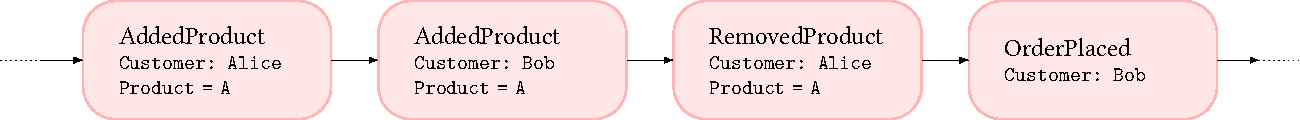
\includegraphics[width=1.0\textwidth]
		{../illustrations/projections2.pdf}

	\caption{
		An excerpt from a hypothetical event log in an online shop.
	}
	\label{fig:projections}
\end{figure}
}

\paragraph{Command}{
In the context of this thesis, a command resembles a requested change to an 
application. A command always results in an event, even in case of a failure.
Commands are typically named in the imperative form (e.g. \cmd{CreateProduct}).
}

\paragraph{Retrospection}
We use the term \emph{retrospection}, to describe the passive (i.e. read-only) 
access of a system's history and prior states.

\paragraph{Retroactive Computing}
With \emph{retroactive computing} (or \emph{retroaction}), we describe the 
interaction with an application's history.  %we describe the active (i.e. writing) 
This includes applying passive retrospective operations, as well as actively
modifying a history. Modifications can be applied through removal or insertion 
operations, as well as a retroactive change of the underlying application 
logic (the source code). This is examined in further detail in Chapters 
\ref{chp:concept} and \ref{chp:programming}.

\section{Command Query Separation (CQS)}
The Command Query Separation principle was first described by Bertrand Meyer 
\mbox{\cite[p.~747]{Meyer1998}} with the intention of improving the handling 
of side effects when creating a program or designing an API. 
A core idea behind this principle is to split access to objects into 
(1) \emph{Queries}, which return information and (2) \emph{Commands}, which 
modify state (Figure \ref{fig:cqs}). Queries should not produce side effects.
An often-mentioned analogy is that a question should never change the answer.

\section{Command Query Responsibility Segregation (CQRS)}
\label{sec:cqrs}

\begin{figure}[t]
	\begin{subfigure}[t]{0.48\textwidth}
	       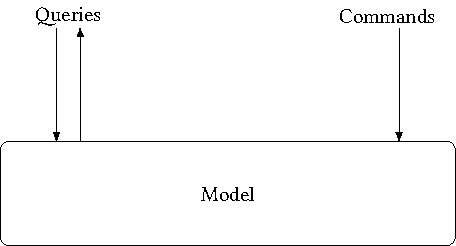
\includegraphics[width=\textwidth]
			{../illustrations/cqs.pdf}
		\caption{
			Command Query Separation (CQS)
		}
		\label{fig:cqs}
	\end{subfigure}
	\quad
	\begin{subfigure}[t]{0.48\textwidth}
	       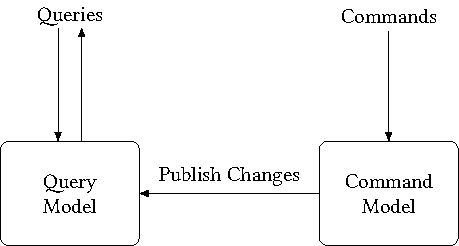
\includegraphics[width=\textwidth]
			{../illustrations/cqrs.pdf}
		\caption{
			Command Query Responsibility Segregation (CQRS)
		}
		\label{fig:cqrs}
	\end{subfigure}
	\caption{Conceptual depiction of both patterns.}
\end{figure}

Command Query Responsibility Segregation is a pattern which was first described 
by Greg Young \cite{Young2013}. In the past, some resources have described it as 
an extension or special case of the Command Query Separation principle, but today 
it is considered a separate pattern with an origin in the CQS principle. 
CQRS states that a different model (i.e. component or object) is used to fulfill 
queries than the model used to fulfill commands (Figure \ref{fig:cqrs}). CQS 
splits responsibilities on the code level, by dividing methods into queries and 
commands; CQRS takes this further and even divides objects into two kinds: 
reading or writing. Young has described this as follows: ``CQRS is simply the 
creation of two objects where there was previously only one'' \cite{Young2010}.

Building an architecture following the CQRS pattern often introduces an 
\emph{eventually consistent} behavior into the system. Since the query and 
command model are separate components, depending on their coupling they might 
not necessarily be in synchronization. 
If they are loosely coupled, the query model does not necessarily contain the 
same data as the command model at every point in time. This characteristic that 
the query model might contain a temporarily inconsistent (i.e. outdated) state, 
which at some point in the future ``eventually'' converges to a consistent state, 
is referred to as eventual consistency.
This eventually consistent behavior becomes especially relevant in distributed 
systems, when the query model(s) are physically separated from the command 
model(s). Brewer's CAP theorem \cite{Brewer1999} postulates that a distributed 
system inevitably has to decide how to handle consistency, since it can only 
ever ensure two of the following three guarantees in case of a network failure:  

\begin{compactenum}
	\item \emph{Consistency}: All participants view the same data.
	\item \emph{Availability}: Each request receives a response.
	\item \emph{Partition Tolerance}: The system continues to operate, 
	even if message loss occurs between arbitrary participants of the
	system. This affects consistency, since participants need to cope
	with the loss of messages. It also affects availability, since each
	participant needs to be able to fulfill requests.
\end{compactenum}

Thus, if a distributed system is built using CQRS as a style of architecture 
and chooses partition tolerance and availability over consistency, the system 
can only provide \emph{eventual} consistency.
Hiding the fact that the system behaves eventually consistent (e.g. by imposing
optimistic assumptions) can be dangerously misleading, since developers and
software components would then operate under false assumptions.
A progressive handling of consistency issues can be seen as a strength of a
distributed ES+CQRS system, since it forces developers to take this very 
consistency behavior -- which is such an integral part of the overall 
architecture -- into account when developing an application. Queries might at 
all times return an outdated result and it is unclear when commands are 
executed. This progressive attitude to issues of large distributed systems has 
spawned a certain kind of attitude and a number of projects in recent years. 
%
The \emph{Reactive Manifesto}~\cite{Boner2014} is a noteworthy document which 
surfaced in 2013. It summarizes key properties behind distributed system design, 
which correspond to event sourcing and CQRS.

\begin{figure}[t]
	\centering
	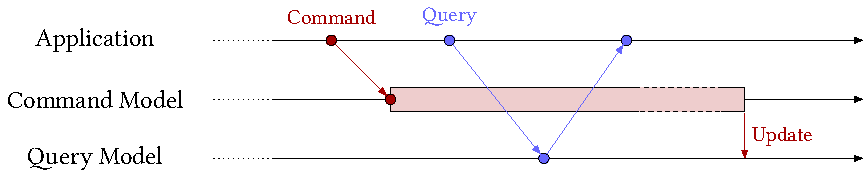
\includegraphics[width=0.8\textwidth]
		{../illustrations/causal-series.pdf}

	\caption{
		In a CQRS architecture, a command and a subsequent
		query do not necessarily possess a causal relationship, since 
		commands are asynchronous and it is unclear when they are
		executed and finished. 
		In the example illustrated above, the query model receives the 
		status update from a finished command after the query has
		already returned. This leads to an eventually consistent
		semantics for queries.
	}
	\label{fig:causal-series}
\end{figure}

A disadvantage of command and query segregation is that it yields a higher 
complexity when building a system and makes it hard to create a causally 
dependent series of commands and events. 
Since commands behave asynchronously and do not return a value, the application 
has no means of knowing when the result of a command is visible.
Thus, a query following a command might return an outdated status.
Subsequent queries, however, will at some point eventually return a consistent 
status. Figure \ref{fig:causal-series} illustrates a typical sequence of commands 
and queries. There are possibilities to circumvent this behavior -- delaying the 
fulfillment of queries until the query model is updated to a certain version 
number for example (as used in conditional requests in 
Eventuate\footnote[1]{\href{https://rbmhtechnology.github.io/eventuate/user\-guide.html\#conditional\-requests}{https://rbmhtechnology.github.io/eventuate/user\-guide.html\#conditional\-requests}}).
%
But it should be noted that these are mitigation techniques which should only 
be used in rare, special cases since they come at the cost of efficiency 
and work against the characteristics of these systems. Instead it is desirable 
for the application to be inherently able to cope with an eventually consistent 
behavior.


\section{Combining ES and CQRS}
\label{sec:es+cqrs}

\begin{figure}[t]
	\centering
	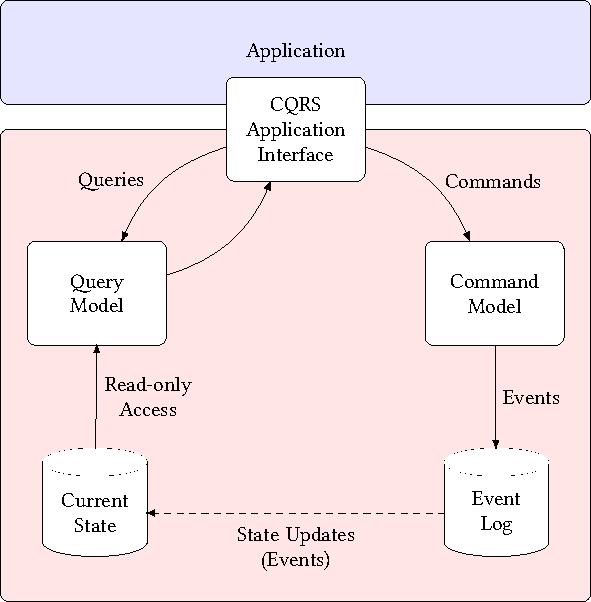
\includegraphics[width=0.5\textwidth]
		{../illustrations/es-cqrs-logic.pdf}

	\caption{
		Architecture of a system which uses event sourcing in 
		combination with CQRS. 
		This illustration is based on a figure from \cite{Erb2014}.}
	\label{fig:escqrs}
\end{figure}

CQRS is a pattern which forms a symbiotic relationship with event sourcing and 
as such is often used in event-sourced architectures.
%
The classification of operations in state-mutating commands and read-only 
queries aligns well with the ideas found in event-sourced systems.
In CQRS, commands represent intentions, which are sent to a command 
processor. There they are processed and yield state changes -- the events.
Events are then appended to the event log and published to query models,
where they eventually update the state as well. Query models fulfill read-only 
requests and can provide a certain view on the data (e.g. a table of accounts 
and their balances). Events are used as the mean to synchronize the models.
%
Thus, commands are then clearly separated from other operations which do not 
result in an append operation to the event log. 
Figure \ref{fig:escqrs} illustrates a typical ES+CQRS architecture: the 
business logic resides in the high level application layer; commands and 
queries hide implementation details of how they are executed. 
Figure \ref{fig:conceptes} depicts a conceptual view with focus on the
internal workings.

The command/query segregation results in characteristics that work well with 
event sourcing. Since events are immutable and are only appended after a 
command has been executed they are the mean to keep data models in 
synchronization. The query models only need to receive new events in order to 
stay consistent with the command model. 
By splitting concerns on an object level, individual optimization of each 
model is supported. 
This is a crucial property for systems with a requirement of scalability,
since the optimization techniques for reads and writes differ.
Segregating the command and query model makes it feasible to scale them 
independently. One technique to optimize for reading operations in a 
distributed system is to replicate the database. These database replicates 
then have to be kept in synchronization, but each of them can then respond 
to requests. A contrasting possibility to optimize for writes, on the other 
hand, is to reduce redundancy (and thus writes) in a database. This can be 
achieved by organizing a single database accordingly, using e.g. normalization 
rules. Further details on the combination of event sourcing and CQRS can be 
found in a work by Hauser \cite{Hauser2014}.

\begin{figure}[h!]
	\centering
	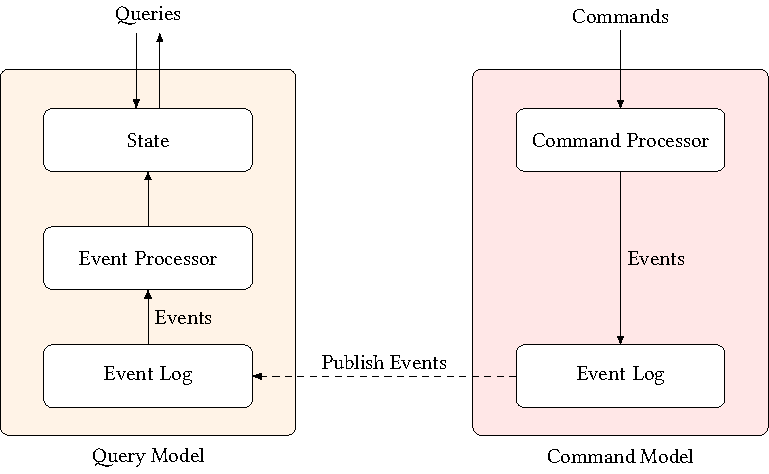
\includegraphics[width=0.67\textwidth]
		{../illustrations/processors.pdf}

	\caption{
		Conceptual view of an event-sourced architecture which takes 
		advantage of the CQRS style.
	}
	\label{fig:conceptes}
\end{figure}

\section{Domain-driven Design (DDD)}
Both, event sourcing and CQRS, are closely related to the idea of domain-driven 
design. The terminology and ideas behind DDD were described by Eric Evans 
\cite{Evans2003} in 2003. At its heart, DDD provides a set of guiding principles 
and building blocks for software development. The core idea here is to put the 
focus of a software project on the domain and the tasks within it. A central part 
when designing a system is the creation of a domain model. Among other components,
this model describes tasks and events of the core domain.
This domain model is created in collaboration with domain experts. In this regard, 
DDD is similar to agile development models, where the collaboration with domain 
experts (or customers) is encouraged as well. 
DDD demands the definition of a common language, the \emph{ubiquitous language}, 
to be used throughout the project. This ubiquitous language is thought to build 
a common view on the domain model amongst team members. Verbs and nouns in the 
language promote a clear understanding of the tasks which need to be fulfilled 
by the system. 
A common language is also thought to prevent misunderstandings and enable anyone 
in a project to talk comprehensibly to any other person in the project, thus 
bringing domain experts and developers together. 

Applying DDD only in this bounded context as well as the usage of high-level 
concepts to abstract from low-level details offer commonalities with the event 
sourcing field.
In an event-sourced system, one usually does not persist all low-level occurring 
events in a system, but rather only relevant domain events in a delimited context. 
DDD is thought to be suited well for systems with complex business rules and a
clearly defined and delimited domain. 
In a simple system, however, DDD may increase complexity to an unnecessary and 
counterproductive level.

The ideas behind event sourcing and CQRS have developed out of DDD. Commands and 
queries in an ES+CQRS system can be modelled using DDD.
This way they have a clear meaning in the domain model and are familiar to 
developers and domain experts. The same holds true for the events which are 
created -- as domain events they fit into the domain model and its logic.
A domain expert describes commands and queries and their internal logic;
an application developer can then access these commands and queries over an
API to implement an application. Since commands and queries abstract from 
domain-specific conditions, working with the system is made easier. 
An application developer does not have to take into account how a command is 
validated or know how it is implemented internally. Complex business logic is 
abstracted through the usage of simplified commands.


\section{Summary}
In this chapter, we detailed the concept of event sourcing. We laid out the
terminology used in this thesis and described the Command Query Responsibility 
Segregation (CQRS) pattern, a common style of architecture for event-sourced 
systems. Furthermore, we examined the symbiotic relationship formed by CQRS 
and event sourcing.

Although we described some of the benefits which event-sourced systems can 
provide, it is important to note that event sourcing is seldom applied to an 
overall system. Indeed, an often found recommendation is to apply this style 
of architecture only within a clearly defined context. The same recommendation 
is often found for CQRS, since the command/query model segregation comes with 
the implication of higher complexity and often an eventually consistent 
behavior. Thus, applying CQRS as a style of architecture is only beneficial 
when the system has requirements for CQRS properties, such as individual 
optimization of the read and write model.
